

This class is part of the four 34x series which constitute the data science core. There is an order that the four classes need to be taken. Below are three plans, the first is over two semesters and hence it is not \emph{not recommended} as it will be a \emph{very} heavy workload. The second is over four semesters and it is the recommended plan as I believe it will allow students to absorb the material more effectively. 

\begin{figure}[htp]
\centering
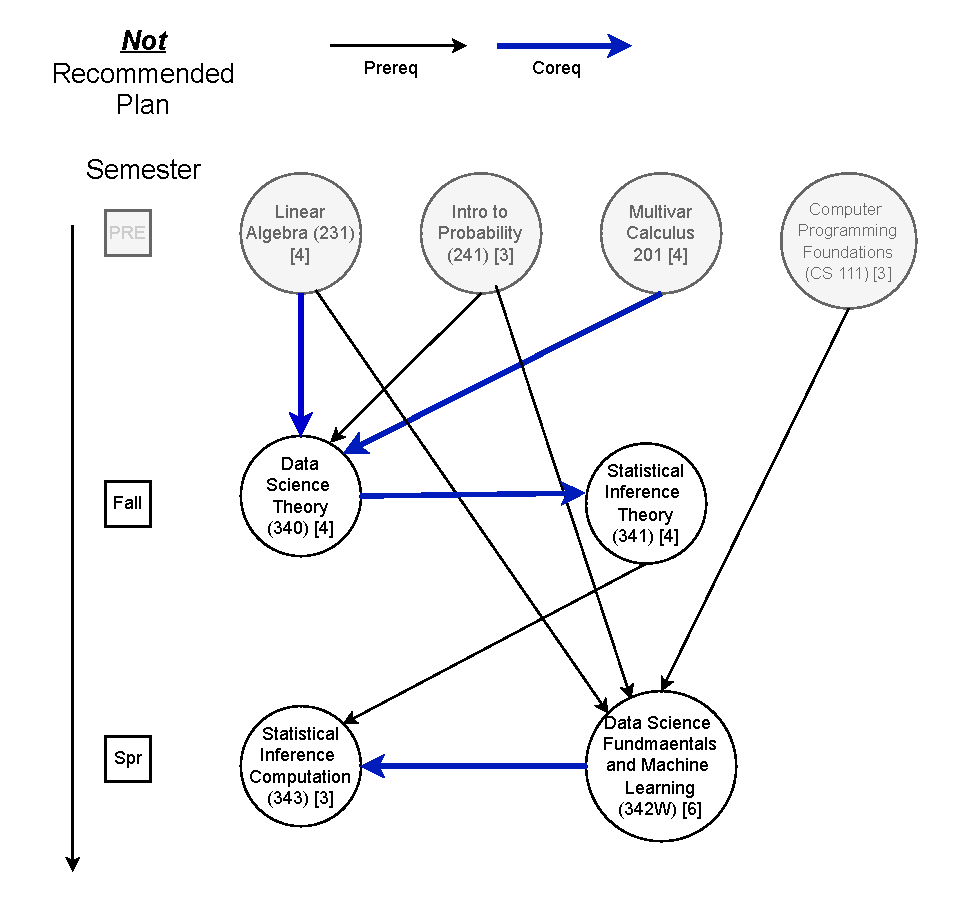
\includegraphics[width=6in]{../../syllabi/not_recommended_plan.pdf}
\label{fig:not_recommended}
\end{figure} 

\begin{figure}[htp]
\centering
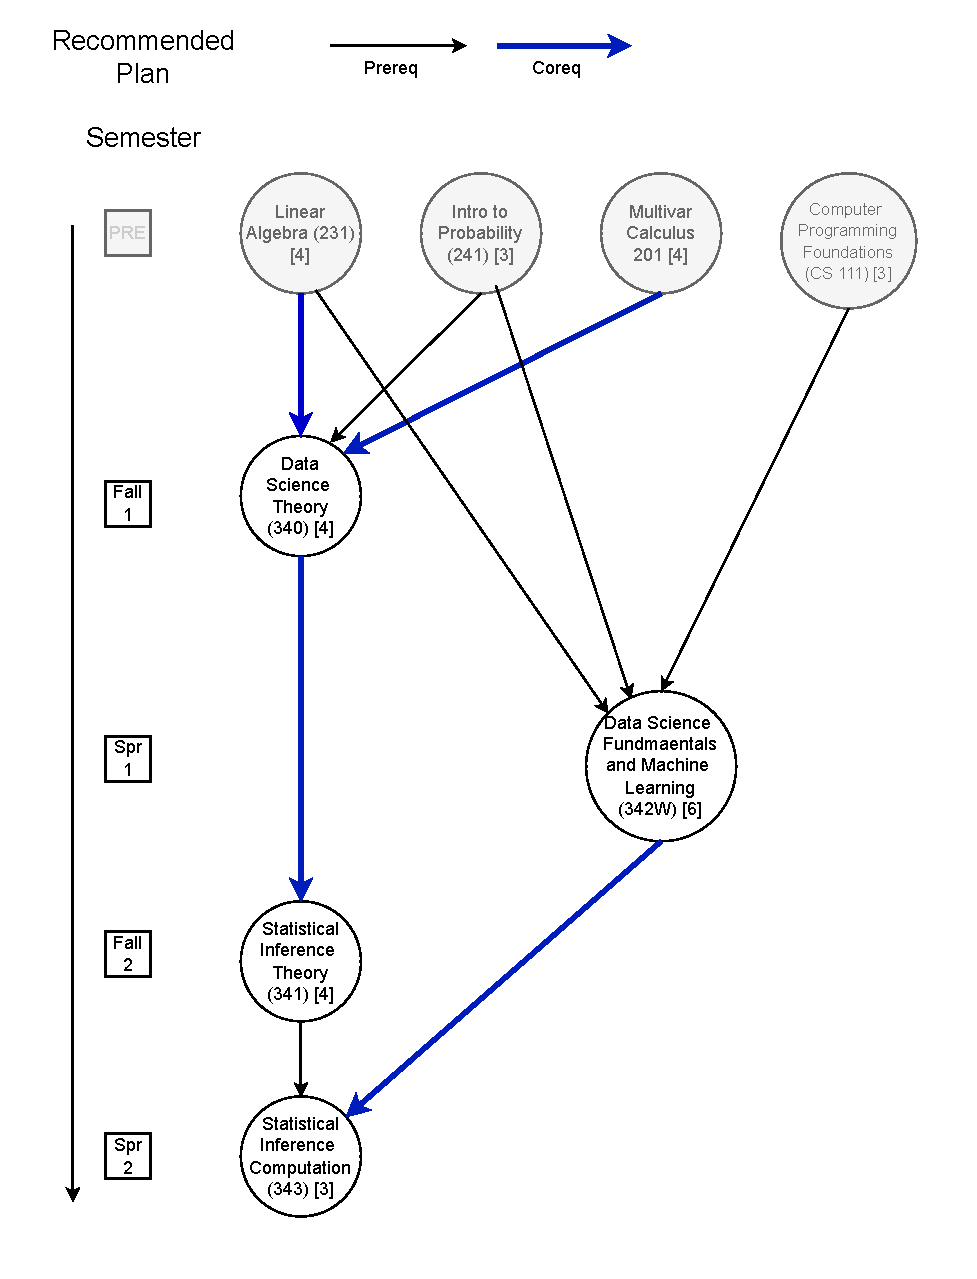
\includegraphics[width=6in]{../../syllabi/recommended_plan.pdf}
\label{fig:recommended}
\end{figure} 

Examining the above, we note that MATH 340 can be taken as a standalone course as a higher-level math elective. It can be thought of as advanced probability following MATH 241. This course is also recommended for students who are considering an actuarial career as this course provides great practice for Exam P.

There is also a third way (not pictured) which is Spring year 1: MATH 342W, Fall year 2: Math 340 and Math 341, Spring year 2: Math 343 which is a middle path with a very difficult Fall semester. 